% ! TEX TS-program = lualatex
% Template for an INTER paper
% To be compiled using lualatex + biber
%
% Author: Cristóbal Tapia Camú
% E-Mail: cristobal.tapia-camu@mpa.uni-stuttgart.de
%
% Package options:
% - unicode-math: use the package unicode-math to render math
% - nounicode-math: deactivate the package unicode-math to render math
% - microtype: use the microtype pacakge to improve overall appearence
%              (Note: If you decide to use microtype beware that some special
%               attention has to be taken to some symbols, e.g. --- (emdash)
%               or -- (endash).
%
%               - To write an emdash (---) with microtype use: \textemdash{}
%               - To write an endash (--) with microtype use: \textendash{}
%
%               Otherwise, everything should work normally.)
%
\documentclass[unicode-math,microtype]{interarticle}
\usepackage{graphicx}
\usepackage{fancyhdr}
\usepackage{lipsum}
\usepackage[subpreambles=true,sort=true]{standalone}
\usepackage{multirow}
\usepackage{verbatim}
\usepackage{booktabs}
\usepackage{bm}
\usepackage{color,soul}
\usepackage[htt]{hyphenat}

\setdefaultlanguage[variant=us]{english}

\sisetup{product-units=power,detect-all}

\bibliography{bib_sample.bib}

\newcommand\comm[1]{\texttt{\textbackslash #1}}

% Title of the paper
\title{Template for INTER papers in Lua\LaTeX\ }
% Authors
\author{%
  Author 1, name + affiliation \and %
  Author 2, name + affiliation %
}

\begin{document}

\maketitle

\keywords{keyword 1\sep keyword 2\sep keyword 3}

\section{Introduction}
This is a template for INTER-papers.
The intention is that the final pdf-file has two of these pages at each page.
This makes it easy to read on a computer screen.
The standard font size (\comm{normalsize}) is therefore \SI{14}{pt}, so it looks like \SI{10}{pt} in the pdf-file.
The typography is predefined to be \texttt{Calibri} (if your are using any Linux distribution, you probably need to install them) and will ensure a homogenous appearance of the proceedings.\par

The title has to be written with the \comm{title} command, and the authors should be put inside the \comm{author} command, separated by \comm{and}.
The title will be autogenerated with the command \comm{maketitle}, which will use the correct typography.\par

Lua\LaTeX\ must be used for the compilation of this file, otherwise the typography will not be displayed correctly (\LaTeX\ and pdf\LaTeX\ do not support the use of true type fonts).\par

\section{Headlines}
Beside the standard font there are 4 levels of headlines, which can be used with the standard commands \comm{section}, \comm{subsection}, \comm{subsubsection} and \comm{paragraph}.

\subsection{Level 2}
This is level 2.

\subsubsection{Level 3}
And this is level 3.

\paragraph{Level 4}
So many levels\ldots this is the last one: level 4.

\section{Equations}
Use any of the standard equation environments, such as \texttt{equation} or \texttt{align} and they will be left-aligned automatically.
%
\begin{equation}
  F=\beta \tan \nu
  \label{eq:eq1}
\end{equation}

The document uses the package \texttt{unicode-math} to render the greek letters in the Calibri font.
If this is causing any problem, it can be deactivated by passing the option \texttt{no-unicode-math} to the class in the preamble: \\
\comm{documentclass[no-unicode-math]\{interarticle\}}.

\subsection{Style}
Symbols (like $F$ and $\beta$) are written in italic, for which either \$\ldots\$ or \comm{textit} can be used.
Functions (like $\tan$) and units (like \si{kN}) in ordinary style.
For the latter, it is recommended to use the package \texttt{stunitx} (e.g.\ \comm{SI\{10\}\{N/mm\^{}2\}} translates into \SI{10}{N/mm^2}, keeping a correct spacing between numbers and units, and the correct typography style).

\section{Figures}
Figures are inserted with the standard environment \texttt{figure}.
The font for the caption is set to be of \SI{12}{pt} (\comm{small}) and in \textit{italic} style.
This is taken care of automatically.
Letters and numbers in the figure should appear no smaller than the figure caption.
The figure is aligned to the left per default.\par

\begin{figure}[htb]
  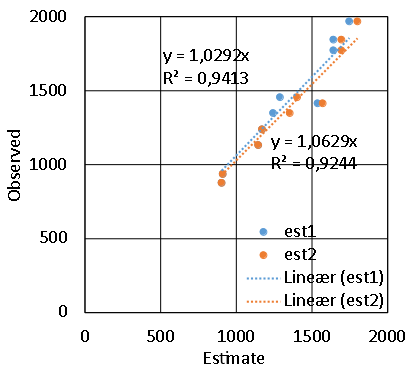
\includegraphics[width=7.6cm]{./img/figure1.png}
  \caption{The observed capacity versus the estimated capacity (\si{N})}%
  \label{fig:figure1}%
\end{figure}


\section{Tables}
Tables should preferably only have horizontal lines.
To insert a new table use the standard \texttt{table} + \texttt{tabular} environments.
The typography of the caption will be taken care of automatically (set to the correct size of \SI{12}{pt} and in \textit{italics}).
The caption should be put before the table.
To insert table-notes, use the package \texttt{threeparttable}.

\begin{table}[htb]
  \small
  \caption{Requirements to sound insulation.}%
  \label{tab:table1}
  \begin{threeparttable}
    \begin{tabular}{lccccc}\toprule
      & Denmark     & Finland & Norway & Sweden & Estonia \\\midrule
      Airborne & \SI{55}{dB}\tnote{*} &         &        &        &         \\
      Impact   &             &         &        &        &         \\\bottomrule
    \end{tabular}
  \begin{tablenotes}
  \item[*] Table note, \SI{11}{pt}.
  \end{tablenotes}
  \end{threeparttable}
\end{table}

\section{Bullet lists}
Use the standard bullet lists from latex with the \texttt{itemize} environment as
\begin{itemize}
  \item sddfd
  \item dfsd
  \item asddf
\end{itemize}

\section{Use of references}
Define the bibliography file with the command \comm{bibliography} at the beginning of the document.
To make an in-text citation use \comm{citet}, which will print like \citet{Isaksson1999}, and use \comm{citep} to make references in parenthesis \citep{Isaksson1999}.
References with two authors will print as \citet{Taylor1991} and for more than two authors ``\emph{et al.}'' form will be used, e.g.\ \citet{Showalter1987}.\par

For publications with no author, e.g.\ standards, use the common names as \citet{EN1995-1-1engl} or \citet{EN14080-2013}.\par

The command \comm{printbibliography} has to be issued at the end of the document, for the reference section to be printed at the end of the paper, as it can be seen in the source code of this example.\par

The format for the \texttt{*.bib} file is \emph{biblatex}, and the backend is \emph{biber}, but can be modified in the \emph{class} file (\texttt{interarticle.cls}).\par

\printbibliography[heading=bibnumbered]

\end{document}
